\documentclass[a4paper,10pt,fleqn, twocolumn]{IEEETran}
\usepackage{amsfonts}
\usepackage{amsthm}
\usepackage{graphicx}
\usepackage{fancyhdr}

\setlength{\parindent}{3em}
\setlength{\oddsidemargin}{0in}
\setlength{\textwidth}{6.5in} % sets 1in left and right margins
\setlength{\topmargin}{0.0in} % change to 0.2in for regular latex
%\setlength{\headheight}{0in}
%\setlength{\footheight}{0.5in}
\setlength{\footskip}{0.5in}
\setlength{\textheight}{9.0in} %sets 1in top and bottom margins
%\renewcommand{\baselinestretch}{1} %set to 1.5 for double spacing.


\newtheorem{Prop}{Proposition}
\newtheorem{lemma}{Lemma}



\newcommand{\br}{{\mathbf r}}
\newcommand{\bA}{{\mathbf A}}
\newcommand{\ba}{{\bf a}}
\newcommand{\bb}{{\bf b}}
\newcommand{\bc}{{\bf c}}
\newcommand{\bC}{{\bf C}}
\newcommand{\bg}{{\bf g}}
\newcommand{\bG}{{\bf G}}
\newcommand{\bd}{{\bf d}}
\newcommand{\be}{{\bf e}}
\newcommand{\bs}{{\bf s}}
\newcommand{\bm}{{\bf m}}
\newcommand{\bn}{{\bf n}}
\newcommand{\bu}{{\bf u}}
\newcommand{\bv}{{\bf v}}
\newcommand{\bw}{{\bf w}}
\newcommand{\bx}{{\bf x}}
\newcommand{\by}{{\bf y}}
\newcommand{\bbf}{{\bf d}}
\newcommand{\bE}{{\bf E}}
\newcommand{\bF}{{\bf F}}
\newcommand{\bL}{{\bf L}}
\newcommand{\bM}{{\bf M}}
\newcommand{\bN}{{\bf N}}
\newcommand{\bS}{{\bf S}}
\newcommand{\bT}{{\bf T}}
\newcommand{\bD}{{\bf D}}
\newcommand{\bX}{{\bf X}}
\newcommand{\bP}{{\bf P}}
\newcommand{\bQ}{{\bf Q}}
\newcommand{\bI}{{\bf I}}
\newcommand{\bR}{{\bf R}}
\newcommand{\bU}{{\bf U}}
\newcommand{\bV}{{\bf V}}
\newcommand{\bW}{{\bf W}}
\newcommand{\bJ}{{\bf J}}
\newcommand{\bB}{{\bf B}}
\newcommand{\bzero}{{\bf 0}}
\newcommand{\bgamma}{{\mbox {\boldmath $\gamma$}}}
\newcommand{\btheta}{{\mbox {\boldmath $\theta$}}}
\newcommand{\bLambda}{{\mbox {\boldmath $\Lambda$}}}
\newcommand{\bPsi}{{\mbox {\boldmath $\Psi$}}}
\newcommand{\bPhi}{{\mbox {\boldmath $\Phi$}}}
\newcommand{\bcA}{{\mbox {\boldmath ${\cal A}$}}}
\newcommand{\bcB}{{\mbox {\boldmath ${\cal B}$}}}
\newcommand{\bcC}{{\mbox {\boldmath ${\cal C}$}}}
\newcommand{\bcD}{{\mbox {\boldmath ${\cal D}$}}}
\newcommand{\bcF}{{\mbox {\boldmath ${\cal F}$}}}
\newcommand{\bcN}{{\mbox {\boldmath ${\cal N}$}}}
\newcommand{\bcS}{{\mbox {\boldmath ${\cal S}$}}}
\newcommand{\bcH}{{\mbox {\boldmath ${\cal H}$}}}
\newcommand{\bcI}{{\mbox {\boldmath ${\cal I}$}}}
\newcommand{\bcR}{{\mbox {\boldmath ${\cal R}$}}}

\title{ Semi-Blind Multiuser Detection }
\date{}
\author{Shu Wang, Sang G. Kim, Li-Hsiang Sun, Hobin Kim,\\
   Suk W. Lee, S. R. Subramanya, Ki Y. Kim and Byung K. Yi\\LGE Mobile Research Center\\San Diego, CA 92131}
\begin{document}
\maketitle

\begin{abstract}
Instead of using the conventional multiuser signal model and/or
the parametric subspace model, we proposed a semiblind signal
model and framework for asynchronous CDMA channels in this paper.
And two semiblind multiuser detectors based on best linear
unbiased estimation (BLUE) and minimum mean squared error (MMSE)
estimation criteria and this framework are developed. Furthermore,
the classic truncated-window scheme is generalized to a
multi-window scheme so that several consecutive bits can be
simultanously detected. The proposed algorithms are simple and
direct, which only require the desired user's timing, amplitude
and signature. No prior knowledge regarding other users is
involved. No search or convergence procedure is employed as in
many other semi-blind or blind detectors. A minimum number of
previously received signals are enough for the proposed framework
to perform detections. Theoretical analysis and computer
simulations are finally presented to support the performance of
the proposed semi-blind multiuser detection schemes.
\end{abstract}

\section{Introduction}
Multiuser detection strategy is a method to minimize the effect of
MAI and solve the near-far problem without a significant reduction
in the signal energies of the strong users in order for the weaker
users to achieve reliable communication. It has been extensively
investigated over the past several years~\cite{Verd98}, since MAI
is the dominant impairment for CDMA systems and exists even in
perfect power-controlled CDMA systems. So far, most multiuser
detection schemes are based on the conventional multiuser signal
model and then detect desired users signal using the minimum
bit-error rate (MBER), least-square (LS) errors,
MMSE~\cite{Lupa89} and/or minimum output energy (MOE) criteria. In
the conventional signal model, a received signal and also
multiuser receiver filter is explicitly composed by all involved
users' amplitudes, timing and spreading signatures, which may be
difficult to be known by semiblind/blind receivers beforehand. On
the other hand, it is known that the adaptive or training
procedure employed by many semiblind/blind multiuser detectors can
cost receivers too much time or computation resource. The
subspace-based parametric multiuser signal model, where each
received signal can be taken as a linear combination of the bases
of signal and noise subspaces, and subspace-based multiuser
detection have attracted many attentions~\cite{Wang98}. Thought
their performance can be well above many previous semiblind/blind
approaches, subspace-based multiuser detectors need compute the
covariance matrix of received signals and separate signal/noise
subspace bases. These may be difficult in many practical
situations when the wireless channel and/or the number of users
experience fast dynamic changes.

In this paper, a semiblind multiuser signal model and multiuser
detection framework for asynchronous CDMA channel is developed
using only desired users' spreading sequence and amplitude and
several previously received signals. Based on this model, we
develop two semiblind multiuser detectors using BLUE and MMSE
criteria instead of the LS criterion which was well discussed
in~\cite{Wang03d,Wang03e}. Different to most existing schemes,
each received asynchronous signal and also semiblind receiver is
taken as a linear combination of the desired user's spreading
sequence, several previously received signals and noise in the
proposed signal model and there is no converging and estimation
procedure employed. The proposed semiblind schemes are simple and
direct. Performance analysis and computer simulations are finally
present to demonstrate their performance.

\section{Data Model and Problem Description}
At first, the conventional $K$-user asynchronous multiuser model
is presented first~\cite{Verd98}. The baseband representation of
the received signal due to the $k$th user is given by

\begin{equation}
\begin{array}{rcl}
r_k(t)&=&\sum\limits_{i=-\infty}^{+\infty}A_k b_k[i]
s_k(t-iT_c-\tau_k)
\end{array}
\end{equation}

\noindent where $b_k[i]$ is the $i$th bit sent by the $k$th user.
We assume that the $\left\{b_k[i]\right\}$ are independent and
identically distributed random variables with
$E\left\{b_k[i]\right\}=0$ and $E\left\{|b_k[i]|^2\right\}=1$. The
parameters $s_k(t)$ denote the normalized signal waveform of the
$k$th user during the interval $[(n-1)T,\ nT]$, $\tau_k$ denotes
the transmission delay from the $k$th user to the base station and
$A_k$ is the amplitude of the received signal of the $k$th user.
The baseband signal at the input of the receiver at the mobile
station is

\begin{equation}
\begin{array}{rcl}
r(t)&=&\sum\limits_{k=1}^{K}r_k(t)+n(t)
\end{array}
\end{equation}

\noindent where $n(t)$ is additive white Gaussian noise (AWGN)
with power spectral density $\sigma_n^2$.

The received signal is synchronized for each user, individually,
passed through the corresponding chip matched filter (CMF), and
sampled at the chip rate $1/T_c$. The vector of the output samples
of the CMF for $k$th user in the $n$th symbol interval can be
expressed as

\begin{equation}\hspace{-0.1in}
\begin{array}{l}
\br_k{[n]}=\left[
\matrix{r_k(nT+T_c+\tau_k)&\ldots&r_k(nT+LT_c+\tau_k)}\right]^{\rm
T}
\end{array}.
\end{equation}

Prior to developing our semi-blind decorrelating detectors, we
first discuss the classic single-truncated-window decorrelating
detector, in which the system is assumed to be chip-synchronous
and the observation window is restricted to one symbol
interval~\cite{Verd98}. Without loss of generality, we consider
the detection of the first user while the other users' signals are
treated as interference. A typical interferer has two consecutive
symbols interfering with the symbol of user $1$ so that the
received signal $\br$ can be conventionally and straightforwardly
expressed by
\begin{equation}\hspace{-0.1in}
\begin{array}{rcl}
\br_1&\hspace{-0.1in}=&\hspace{-0.1in}A_1b_1{[n]}\bs_1+\sum\limits_{k=2}^{K}A_k\left\{b_k{[n-1]}
\bs_{k-}+b_k{[n]} \bs_{k+}\right\} + \bn\\
&\hspace{-0.1in}=&\hspace{-0.1in}\bS_1\bA_1\bb_1+\bn
\end{array} \label{r}
\end{equation}
\noindent where $\bs_{k_-}$ and $\bs_{k_+}$ are effective
signature sequences or partial signature sequences that are
completely determined by the spreading sequences $\bs_k$ and the
delays relative to the first user $\tau_{k1}=\tau_k-\tau_1$, $\bn$
is an $L$-dimension Gaussian vector with independent
$\sigma_n^2$-variance components, $L \geq 2K-1$, and

\begin{equation}\hspace{-0.6in}
\begin{array}{l}
\bS_1=\left[\matrix{\bs_1&\bs_{2-}&\bs_{2+}&\ldots&\bs_{K-}&\bs_{K+}}\right]\\
\end{array}\label{S1}
\end{equation}
\begin{equation}\hspace{-0.0in}
\begin{array}{l}
\bA_1=\mbox{diag}\left\{\matrix{A_1&A_2&A_2&\ldots&A_K&A_K}\right\}\\
\end{array}
\end{equation}
\begin{equation}\hspace{-0.1in}
\begin{array}{l}
\bb_1=\left[\matrix{b_1[n]&b_2[n-1]\ b_2[n]&\ldots&b_K[n-1]\
b_K[n]}\right]^{\rm T}.
\end{array}
\end{equation}

The classic single-truncated-window decorrelating detector
actually performs the following operation

\begin{equation}
\begin{array}{rcl}
\hat{\bb}_1&=&\mbox{sgn}\{\bS_1^{+}\br_1\}
\end{array}
\end{equation}

\noindent where $[\cdot]^+$ denotes generalized inverse. The
single-truncated-window decorrelating detector is designed to
completely eliminate MAI caused by other users, which is achieved
at the expense of enhancing the ambient noise. However, there are
some desirable features of this multiuser detector. It does not
require knowledge of the received amplitudes of all users, but it
does require $\bS_1^+$ and the delays of all users. It can readily
be decentralized in the sense that the demodulation of each user
can be implemented completely independently.

\section{Semi-blind Signal Model And Framework}
\begin{figure} \center{
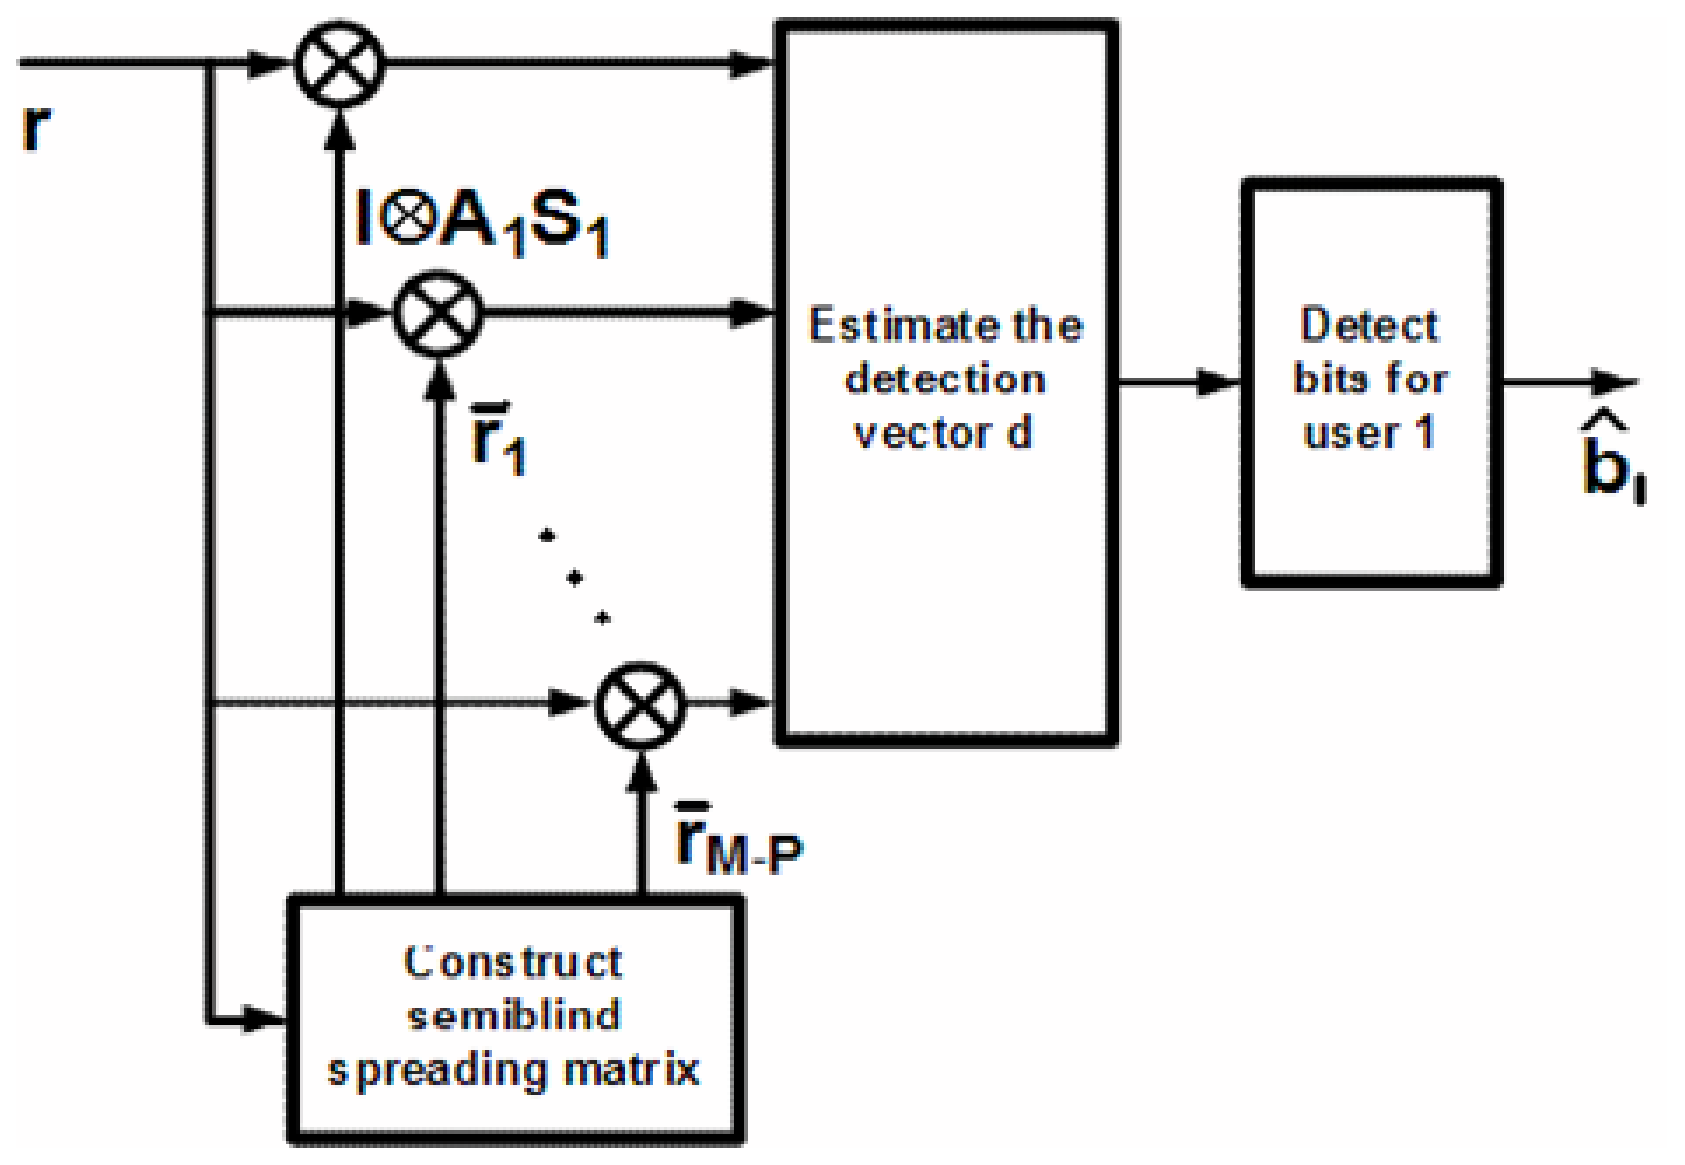
\includegraphics[width=2.5in]{SBMUDstruct2.eps}
\caption{Semiblind Multiuser detection models.  }
}\label{MUD_model}
\end{figure}
Though the conventional multiuser signal model in (\ref{r})
provides an accurate and straightforward description of the
received signal $\br$, it may be difficult to be directly used in
semiblind/blind multiuser detection since the unknown original
spreading sequences matrix is used. We extend the synchronous
semiblind detection idea in~\cite{Wang03d,Wang03e} and define a
new asynchronous $PL\times M$ semi-blind signal signature matrix
$\bcS$ for user $1$ in Fig.~\ref{MUD_model} as

\begin{equation}
\begin{array}{rcl}
\bcS&=&[\matrix{\bI_P \otimes (A_1\bs_1)&\bar{\br}_{1}&\bar{\br}_{2}&\ldots&\bar{\br}_{M-P}}]\\
 &=&\bS\bar\bA\bB + \bar{\bN}
\end{array} \label{S}
\end{equation}

\noindent where the $PL\times (PK+K-1)$ matrix
\begin{equation}
\begin{array}{rcl}
\bS&=&[\matrix{\bar{\bS}_1&\bar{\bS}_2&\bar{\bS}_3&\ldots&\bar{\bS}_K}]
\end{array} \label{S0}
\end{equation}

\noindent is a multi-window version of the original signature
matrix $\bS_1$ with

\begin{equation}
\begin{array}{rcl}
\bar{\bS}_1&=&\mbox{diag}\{\matrix{\bs_1&\bs_1&\ldots&\bs_1}\}_{PL\times
P}
\end{array}
\end{equation}

\noindent and

\begin{equation}
\begin{array}{rcl}
\bar{\bS}_k&=&\mbox{diag}\{\matrix{\bs_{k_-}&\bs_k&\ldots&\bs_k&\bs_{k_+}}\}_{PL\times
(P+1)}
\end{array},
\end{equation}

\noindent the $(PK+K-1)\times (PK+K-1)$ diagonal matrix
\begin{equation}
\begin{array}{rcl}
\bar\bA&=&\mbox{diag}\{\matrix{\bar{\bA}_1&\bar{\bA}_2&\ldots&\bar{\bA}_K}\}
\end{array}
\end{equation}

\noindent denotes a multi-window amplitude diagonal matrix with

\begin{equation}
\begin{array}{rcl}
\bar{\bA}_1&=&\mbox{diag}\{\matrix{A_1&A_1&\ldots&A_1}\}_{P\times
P}
\end{array}
\end{equation}

\noindent and

\begin{equation}
\begin{array}{rcl}
\bar{\bA}_k&=&\mbox{diag}\{\matrix{A_k&A_k&\ldots&A_k}\}_{(P+1)\times
(P+1)}
\end{array},
\end{equation}

\noindent $\bar{\br}_i$ are several previously received vectors of
length $P$ symbols,
\begin{equation}\hspace{-0.0in}
\begin{array}{rcccl}
 \bB &=&\left[\matrix{\bC \cr \matrix{\mathbf{0}& \tilde{\bD}}
 }\right]
 &=&\left[\matrix{\bI_P& \bar{\bD} \cr \mathbf{0}& \tilde{\bD}
 }\right],
\end{array}\label{B}
\end{equation}
with the $PL\times(M-P)$ multi-window bits matrix $\bD =
[\bar{\bD}^{\rm T}\ \tilde{\bD}^{\rm T}]^{\rm T}$, in which
$\bar{\bD}$ is a known $(M-P)\times P$ vector consisting of
previously detected bits for the desired user.
$\mbox{rank}\{\bB\}=PK+K-1$ and
$\mbox{rank}\{\tilde{\bD}\}=PK+K-P-1$. The $PL\times M$ matrix
$\bar{\bN}=[\mathbf{0}\ \tilde{\bN}]$ denotes the multi-window
noise matrix. $\otimes$ denotes the Kronecker product and we
maintain $PL\geq M\geq PK+K-1$.

Using (\ref{r}) and (\ref{S}), the semiblind representation of the
current received signal vector $\br$, which is of length $P$
symbols, is given by
\begin{equation}\hspace{-0.2in}
\begin{array}{l}
\br=[\matrix{\br_1[n]^{\rm T}&\br_1[n-1]^{\rm T}&\ldots&\br_1[n-P+1]^{\rm T}}]^{\rm T}\\
\hspace{0.1in}=\bcS\bd + \bar{\bn} \label{rn}
\end{array}
\end{equation}
\noindent where the $M \times 1$ vector $\bd$ denotes the new
detection vector and is defined as

\begin{equation}
\begin{array}{rcl}
\bd&=&\bB^+\bar\bb_1
\end{array} \label{DetectorVector}
\end{equation}

\noindent and $\bar{\bn}$ is the new noise vector and defined as
\begin{equation}
\begin{array}{rcl}
\bar{\bn}&=&\bn-\bar{\bN}\bB^{+}\bar\bb_1
\end{array} \label{new_noise}
\end{equation}
\noindent With (\ref{B}) and (\ref{DetectorVector}), the bits
vector $\bar{\bb}$ which consists of the bits sent by user 1 at
$P$ consecutive symbol intervals $t=n-P+1$, $n-P+2$, $\ldots$, $n$
can be obtained by
\begin{equation}
\begin{array}{rcl}
\bar{\bb}_1&=& \bC\bd
\end{array}. \label{bn_estimation}
\end{equation}

\section{Semi-Blind Multiuser Detection}
After defining the semi-blind signature matrix $\bcS$ in
(\ref{S}), the conventional multiuser signal model (\ref{r}) be
transformed into (\ref{rn}). The difference between them is the
information bit vector $\bb$ is replaced by the detection vector
$\bd$ and the original AWGN noise vector $\bn$ is replace by the
new noise vector $\tilde{\bn}$ besides $\bcS$ has already been
known beforehand. On the other hand, the relationship between
$\bd$ and $\bb$, which can be expressed in (\ref{bn_estimation}),
makes the semiblind detection possible. The next question then is
how to efficiently estimate $\bd$.

Since it is difficult to determine the optimal minimum variance
unbiased estimator (MVU) for $\bd$, it is reasonable to resort to
suboptimal estimators. In~\cite{Wang03d,Wang03e}, three LS-based
semiblind detectors were proposed with different assumptions
regarding the noise item $\bar{\bN}$ in $\bcS$. There is no
channel/sequence estimation involved in them. In the following,
two estimation schemes based on BLUE and MMSE criteria are
proposed using some statistical information regarding $\bd$ and
$\bar\bn$

\subsection{Best Linear Unbiased Detection}
We assume the linear structure
\begin{equation}
\begin{array}{rcl}
{\bbf}_{\rm BLU}&=&\bW_{\rm BLU}^{\rm T}\br
\end{array}
\end{equation}
\noindent for this so-called best linear unbiased estimator
(BLUE). Matrix $\bW_{\rm BLU}$ is designed such that: 1) $\bcS$
must be deterministic, 2) $\bar{\bn}$ must be zero mean with
positive definite known covariance matrix $\bC_{\bar{\bn}}$, 3)
${\bbf}_{\rm BLU}$ is an unbiased estimator of $\bbf$, 4) and the
error variance for each of the $M$ parameters is minimized as
\begin{equation}
\begin{array}{rcl}
\bW_{\rm BLU}&=&\min\limits_{\bW_{\bbf}}
\mbox{var}\left\{\bW_{\bbf}^{\rm T}\br\right\}
\end{array}
\end{equation}
\noindent In this way, ${\bbf}_{\rm BLU}$ will be unbiased and
efficient, within the class of linear estimators, by design. The
resulting best linear unbiased estimator is (Gauss-Markov
Theorem):
\begin{equation}
\begin{array}{rcl}
{\bbf}_{\rm BLU}&=&(\bcS^{\rm
T}\bC_{\bar{\bn}}^{-1}\bcS)^{-1}\bcS^{\rm
T}\bC_{\bar{\bn}}^{-1}\br\ .
\end{array} \label{BLUE}
\end{equation}
\noindent The covariance matrix of ${\bbf}_{\rm BLU}$ given by
\begin{equation}
\begin{array}{rcl}
{\bC}_{\bbf_{\rm BLU}}&=&(\bcS^{\rm
T}\bC_{\bar{\bn}}^{-1}\bcS)^{-1}
\end{array}.
\end{equation}
\noindent Though the PDF of $\bB$ may be determined, the PDF of
$\bB^{+}$ is largely unknown. This makes it is hard to calculate
the closed-form solution of $\bC_{\bbf}$ and $\bC_{\tilde{\bn}}$.
However, with Girko's Law, when $\alpha=(K-G)/(M-G)$ is fixed,
$K$, $M$ $\rightarrow\infty$, the diagonal element of
$\frac{1}{M-G}\tilde{\bD}^+\tilde{\bb}\tilde{\bb}^{\rm
T}\tilde{\bD}^{\rm +T}$ may be approximated
by~\cite{Muller,Hanly90}
\begin{equation}
\begin{array}{rcl}
\lim\frac{1}{M-G}\left[\tilde{\bD}^+\tilde{\bb}\tilde{\bb}^{\rm
T}\tilde{\bD}^{\rm +T}\right]_{ii}^{-1}&=&1-\alpha
\end{array}.
\end{equation}
\noindent So, $\bC_{\bbf}$ can be decided by
\begin{equation}
\begin{array}{rcl}
\bC_{\bbf}&=&\left[\matrix{\frac{2M-K-G}{M-K}\bA_1^2&\bzero^{\rm
T}\cr\bzero&\frac{1}{M-K}\bI}\right]
\end{array},
\end{equation}
\noindent where $\bA_1=\mbox{diag}\{\ba_1\}$,
\begin{equation}
\begin{array}{rcl}
\bC_{\bar\bn}&=&\sigma^{2}\frac{2M-K-G}{M-K}\bI
\end{array}\label{noise_var_new}
\end{equation}
\noindent and the bit vector for user $1$ can be detected by
\begin{equation}
\begin{array}{rcl}
\hat{\bb}_1&=&\mbox{sign}\left\{\bG(\bcS^{\rm
T}\bcS)^{-1}\bcS^{\rm T}\br\right\}
\end{array}
\end{equation}

\subsection{Minimum Mean Square Detection}
Now we estimate $\bbf$ based on MMSE criterion. This class of
estimators are generically termed Wiener filter. Given
measurements $\br$, the MSE estimator of $\bbf$, ${\bbf}_{\rm MS}
= f( \br )$, minimizes the mean-squared error $J_{\rm
MSE}=E\{||\bbf-\hat{\bbf}||_2^2\}$. The function $f(\br)$ may be
nonlinear or linear and its exact structure is determined by
minimizing $J_{\rm MSE}$. When $\bbf$ and $\br$ are jointly
Gaussian, the linear estimator $\bW_{\rm MMS}$ that minimizes the
mean-sqared error is (Bayesian Gauss-Markov Theorem)
\begin{equation}
\begin{array}{rcl}
{\bbf}_{\rm MMS}&=&(\bC_{\bbf}^{-1}+\bcS^{\rm
T}\bC_{\bar{\bn}}^{-1}\bcS)^{-1}\bcS^{\rm
T}\bC_{\bar{\bn}}^{-1}\br
\end{array} \label{MSE}
\end{equation}
\noindent and the bit vector for user $1$ can be detected by
\begin{equation}\hspace{-0.05in}
\begin{array}{l}
\hat{\bb}_1=\mbox{sign}\left\{\bG(\bC_{\bbf}^{-1}+\bcS^{\rm
T}\bC_{\bar{\bn}}^{-1}\bcS)^{-1}\bcS^{\rm
T}\bC_{\bar{\bn}}^{-1}\br\right\}
\end{array}
\end{equation}

\section{Performance Analysis}
\subsection{Multiuser Signal Model Comparasion}
The comparison between the proposed asynchronous multiuser signal
mode and the classic single-window signal model is given in the
following table. A similar comparison for the synchronous case can
be found in~\cite{Shen05}.

\begin{figure*}[t]\label{ModelComp}
\begin{center}
\center{}
\begin{tabular}{lcc}
Parameters&The proposed model&The classic model\\
\hline
Common/Shared& dedicated& shared\\
Required Timing Information&$\mbox{only user 1}$ & $\mbox{all users}$\\
Required Amplitude Information&$\mbox{only user 1}$ & $\mbox{all users}$\\
Required Spreading Sequences&$\mbox{only user 1}$ & $\mbox{all users}$\\
 \hline
Input Vector&$\bf{r}\ -\ 1\times\rm PL$&$\bf{r}_1\ -\ 1\times\rm L$\\
Output Vector &$\bar\bb_1\ -\ 1\times\rm P$&$\bb_1\ -\ 1\times\rm K$\\
Num of Detected Bits& P & 1\\
Spreading Matrix &$\bcS\ -\ \rm PL\times\rm M$&$\bS\ -\ \rm L\times\rm K$\\
Amplitude Matrix &$\rm N/A$&$\bf{A}\ -\ \rm K\times\rm K$\\
Noise Vector &$\bar\bn\ -\ 1\times\rm PL$&$\bn\ -\
1\times\rm L$\\

 \hline
\end{tabular}
\end{center}
\end{figure*}

\subsection{Comparasion with The Classic Decorrelator}

When there is no noise in $\bcS$, $\bG$ is accurately known
beforehand and $P=1$, there is the following relationship between
the user $1$'s BLU detector $\bw_{\rm BLU}$ and the decorrelator
$\bw_{\rm DD}$.

\begin{equation}
\begin{array}{rcccl}
\bw_{\rm BLU}&=&\bG(\bcS^{\rm T}\bcS)^{-1}\bcS^{\rm
T}&=&A_1^{-1}\bw_{\rm DD}
\end{array}
\end{equation} \label{wN0}

\noindent On the other hand, $\bw_{\rm DD}$ can be taken as a
special case of $\bw_{\rm BLU$ with $\bB =\bI$ and $P=1$. At this
time, the bit-error-rate of the user 1 

\begin{equation}
\begin{array}{rcl}
P_{e}&=&Q\left({A_1\over \sigma_{n}\sqrt{R_{11}^+}}\right)
\end{array}
\end{equation}

\noindent where $R_{11}^+$ is a shorthand for $(\bR^{-1})_{11}$,
the $1$th row and $1$th column element in the matrix
$\bR^{-1}=(\bS^T\bS)^{-1}$.

Thus, the presented LS semi-blind detector at this time achieves
the maximum near-far resistance as the classic
single-truncated-window decorrelating detector does.


\subsection{The Relationship between $\tilde{\bn}$ and $\bn$}

The mean of the semi-blind noise item $\tilde{\bn}$ in
(\ref{new_noise}) given by

\begin{equation}
\begin{array}{rcccl}
\tilde{m}&=&E\{\tilde{\bn}\}&=&0
\end{array}
\end{equation}

The variance of $\tilde{\bn}$ satisfies the following inequation

\begin{equation}\hspace{-0.2in}
\begin{array}{rcl}
\max var\{\tilde{\bn}\}&=&\max E\{(\tilde{\bn}-\tilde{m})^2\}\\
&\leq&\sigma_n^2+(P+1)(K-1)\|\tilde{\bD}^+\|_2^2\sigma_{\bar{n}}^2
\end{array} \label{noise_mean}
\end{equation}
\noindent where $\max\{\star\}$ denotes the maximum item in the
vector $\star$ and $\sigma_{\bar{n}}^2$ is the power of the noise
item $\bar{\bN}$ in the semi-blind signature matrix $\bcS$.

It is easy to see that the new semi-blind noise item $\tilde{\bn}$
is enhanced compared to the former noise item $\bn$. This
enhancement is because there is the noise $\bar{\bN}$ existing in
the semi-blind signature matrix $\bcS$.

\subsection{AME and Near-Far Resistance}
A commonly used performance measure for a multiuser detector is
asymptotic multiuser efficiency(AME) and near-far
resistance~\cite{Verd98}. Since the proposed algorithms converges
to the conventional decorrelating detector as $\sigma\rightarrow
0$, their AME and near-far resistance are identical to those of
the decorrelating detector:
\begin{equation}
\begin{array}{rcl}
\bar{\eta}_k&=&\frac{1}{\bR_{kk}^{+}}
\end{array}.
\end{equation}
\subsection{CRLB for $\bbf$ Estimation}
The Cram\'{e}r-Rao Lower Bound (CRLB) is given by the inverse of
the Fisher information matrix (FIM). Providing the blind spreading
matrix $\bcS$ is known beforehand, we first define the parameter
vector $\mathbf{\phi} = \left[\bar{\sigma}^{2}\ \bbf^{\rm
T}\right]^{\rm T}$, where $\bar{\sigma}^{2}
=(1+\frac{M-G}{M-K})\sigma^{2}$, for computing the FIM, which is
defined by
\begin{equation}
\begin{array}{rcl}
{\rm FIM} &=& {\rm E} \left\{ \left( \frac{\partial \ln{\cal
L}}{\partial \mathbf{\phi}} \right) \left( \frac{\partial \ln{\cal
L}}{\partial \mathbf{\phi}} \right)^{\rm H} \right\} \label{fim}
\end{array}
\end{equation}
\noindent where $\ln{\cal L}$ is the log-likelihood function given
by
\begin{equation}
\begin{array}{rcl}
\ln{\cal
L}&=&C-L\ln\bar{\sigma}^2-\frac{1}{2\bar{\sigma}^2}\parallel\mathbf{e}\parallel_2^2
\end{array},\label{logl}
\end{equation}
\noindent $C$ is a constant and $\mathbf{e}=\br-\bcS\bbf$.
Providing $\bcS$ is known, the closed-form CRLB expression of
$\bbf$ is then given by
\begin{equation}
\begin{array}{rcl}
{\rm CRLB}(\bbf\ |\ \bcS) &
=&(1+\frac{M-G}{M-K})\sigma^{2}(\bcS^{\rm T}\bcS)^{\rm +}
\end{array}.\label{CRLB_f}
\end{equation}
\noindent From (\ref{CRLB_f}), it shows that the accuracy of
estimating $\bbf$ may increase with increasing $M$.


\section{Computer Simulations}

In this section, various computer simulations and analytical
results are presented. In the computer simulations, two users are
sending the signals in asynchronous CDMA system. The spreading
gain $g=24$. the covariance matrix between these two users are
$\bR$.

\begin{equation}
\begin{array}{rcl}
\bR&=&\left[\matrix{\bs_1^T\cr\bs_{2_-}^{T}\cr\bs_{2_+}^{T}}\right][\matrix{\bs_1&\bs_{2_-}&\bs_{2_+}}]\\
    &=&\left[\matrix{1.0000&-0.6250&-0.0417\cr
                    -0.6250& 0.8750&      0\cr
                    -0.0417&      0& 0.1250}\right]
\end{array}
\end{equation}

\noindent and the channel is AWGN channel. We do the simulations
with $P=1$, $2$, $3$, $4$, $5$, $7$ and $9$. Correspondingly, the
number of columns in the semi-blind signature matrix is
$M=(P+1)\times K-1$. We will compare our algorithms with
single-user matched filter (MF) detector and the
single-truncated-window decorrelating detector (DD).

\section{Conclusions}

In this paper, we presented the one-shot LS and MLS semi-blind
decorrelating detectors with the multiple consecutive truncated
windows. In these two semi-blind multi-windows decorrelating
detector, besides the signature and timing of the desired user,
the amplitude of this user is also required. This is why they are
called semi-blind detectors. In the theoretical analysis and
computer simulations, as we may see, when there is no noise in the
semi-blind signature matrix $\bcS$ and $P=1$, the classic
single-truncated-window decorrelating detector is just one special
case of the presented LS semi-blind detector with $\bB=\bI$. And
when there is no noise in the semi-blind signature matrix, the
performance of the LS semi-blind detector with multiple windows is
better than that with $P=1$ and the classic
single-truncated-window decorrelating detector.

These two semi-blind decorrelating detectors are simple and
direct. No searching or converging procedure is required as in
other semi-blind/semi-blind detectors.

\bibliographystyle{unsrt}
\bibliography{J-AsynchSemiBlindDetector10}
\end{document}
